\documentclass[a4paper, 12pt]{scrreprt}
\usepackage[german]{babel}
\usepackage[german]{translator}
\usepackage[utf8]{inputenc}
\usepackage[T1]{fontenc}
\usepackage{ae}
\usepackage[bookmarks,bookmarksnumbered]{hyperref}
\usepackage{graphicx}
\usepackage{color}
\usepackage[dvipsnames]{xcolor}
\usepackage{booktabs}
\usepackage{longtable}
\usepackage{listings}
\usepackage{tabularx}
\usepackage[left=2.00cm, right=2.50cm, bottom =2.53cm]{geometry}
\usepackage{ pdflscape}
%\usepackage{pdfpages}
%\usepackage[section]{placeins}


\newcommand{\col}[2]{\textcolor{#1}{#2}}

% Zeilenhöhe bei Tabellen
\newcommand{\zh}[1]{\parbox[0pt][#1][c]{0cm}{}}

\begin{document}
	\thispagestyle{plain}
	
	\begin{titlepage}
		\begin{center}
			\begin{figure}[ht]
				\centering
				
\includegraphics[width=0.66\textwidth, angle=0]{logo/name_blau_ofCourse.jpg}
			\end{figure}
			
			\begin{title}
				\title{\Huge{\textbf{Kurseinheiten-Manager \\ \ \\ \ \\ \
							Handbuch Installation\\ 
							\ \\}}}
				
			\end{title}
			\hspace{3cm}
			
			Software Engineering Praktikum \\
			Sommersemester 2015\\
			Universität Passau\\
			
			
			Betreuer: Andreas Stahlbauer \\
        	\hspace{1,5cm}\\
        	Version: 1.0 \\
        	\hspace{1,5cm}\\
        	Datum: 26.06.2015\\[50pt]
        	Team 3 \\
    
		    \ \\
        
        \begin{tabular}{ | l | l | l | l |}
        	\hline
        	\textbf{Matrikelnummer} & \textbf{Name} & \textbf{Phase} & \textbf{E-Mail}  \\ \hline
        	63097 & Katharina Hölzl & Pflichtenheft & hoelzlka@fim.uni-passau.de \\ \hline
        	64504 & Ricky Strohmeier& Entwurf & strohric@fim.uni-passau.de  \\ \hline
        	61085 & Sebastian Schwarz & Feinspezifikation & sebastian@nrschwarz.de \\ \hline 
        	64080 & Tobias Fuchs & Implementierung  &  fuchstob@fim.uni-passau.de\\ \hline
        	58379 & Patrick Cretu  &  Validierung & cretu@fim.uni-passau.de \\ \hline
        \end{tabular}
        
        \ \\
        \ \\
       
        
        
    \end{center}
\end{titlepage}


% Platzierung des Inhaltsverzeichnisses
\tableofcontents
\chapter{Benötigte Software}
Für die Vorbereitung, Einrichtung und Inbetriebnahme der Webapplikation \textbf{ofCourse} wird folgende Software benötigt.
\begin{itemize}
	\item Java SE Development Kit 8
	\item PostgreSQL Datenbank
	\item Apache Tomcat 8
	\item 7Zip
	\item Webbrowser(z.b. Firefox 38)
\end{itemize}
\chapter{Einrichtung des Tomcat Servers}

\chapter{Vorbereitung von ofCourse}
\chapter{Deployment ofCourse}
\chapter{Erster Login}
Geben Sie in ihren Browser folgende URL ein:
\begin{center}
	{\it http://localhost:8003/OfCourse/}
\end{center}
Sie befinden sich nun auf der Startseite von \textbf{ofCourse}.
\begin{figure}[h]
\centering
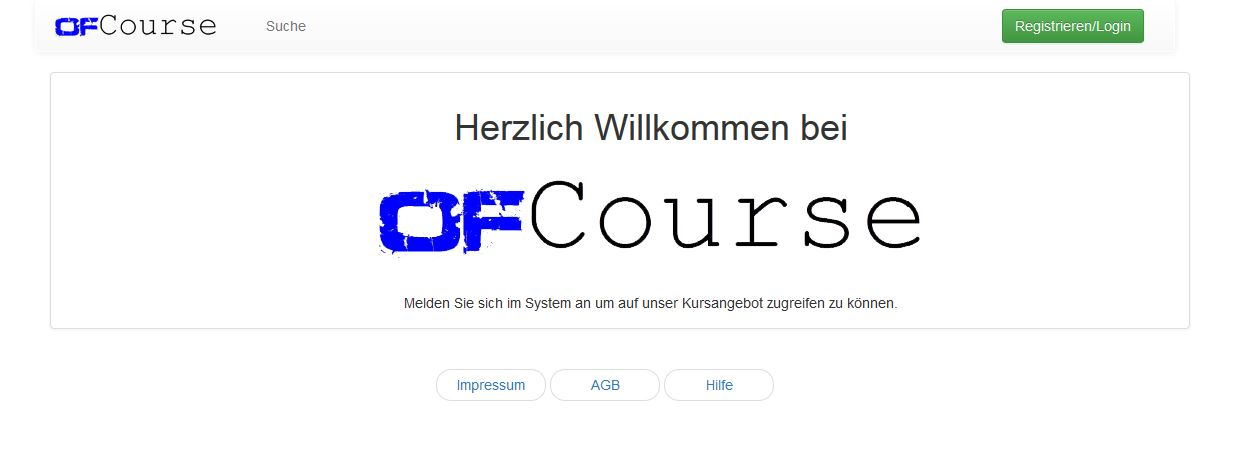
\includegraphics[width=0.8\linewidth]{Grafiken/indexPage}
\caption[]{Startseite von ofCourse}
\label{fig:indexPage}
\end{figure} \ \\
Durch Betätigen des  gruenen Buttons \textbf{Registrieren/Login} links oben auf der Startseite werden Sie auf die Anmeldeseite weitergeleitet.
\begin{figure}[h]
\centering
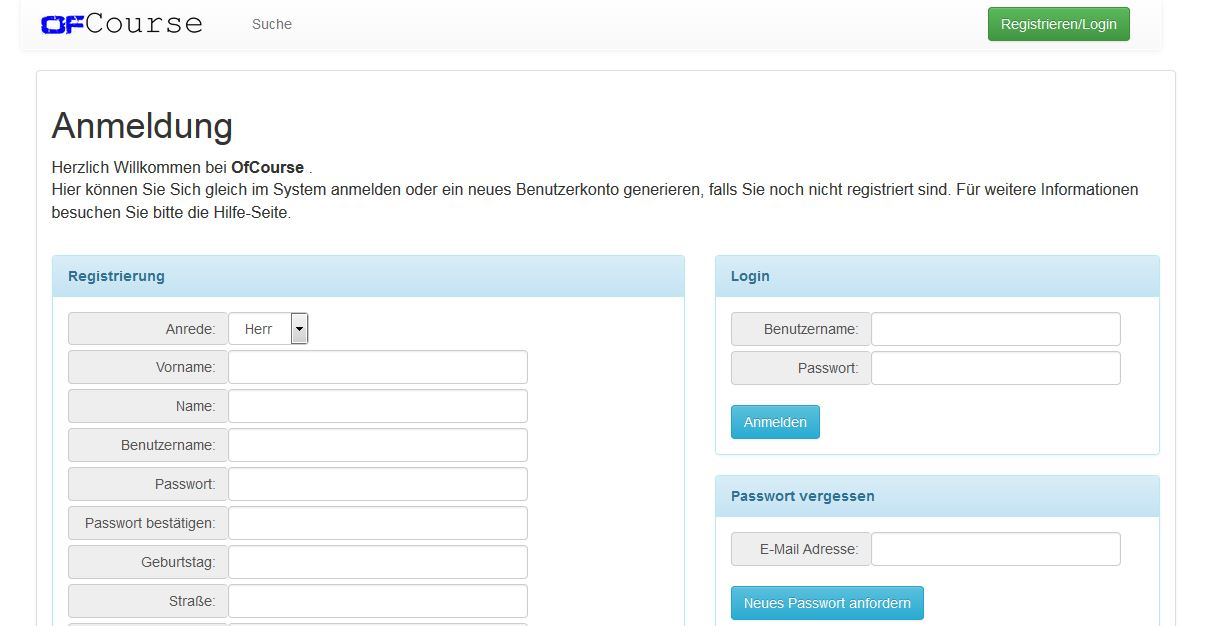
\includegraphics[width=0.8\linewidth]{Grafiken/loginPage}
\caption{Ausschnitt der Anmeldeseite}
\label{fig:loginPage}
\end{figure} \newpage
\ \\
Füllen Sie nun die Felder {\it Benutzername} und {\it Passwort} mit folgenden Daten aus und Betätigen Sie den \textbf{Anmelden} Button.
\begin{center}
	Benutzername: {\it admin1}\\
	Passwort: {\it password}
\end{center}
Sie werden nun auf die \textbf{Meine Kurse} Seite weitergeleitet und sind nun erfolgreich im System angemeldet.
\begin{figure}[h]
\centering
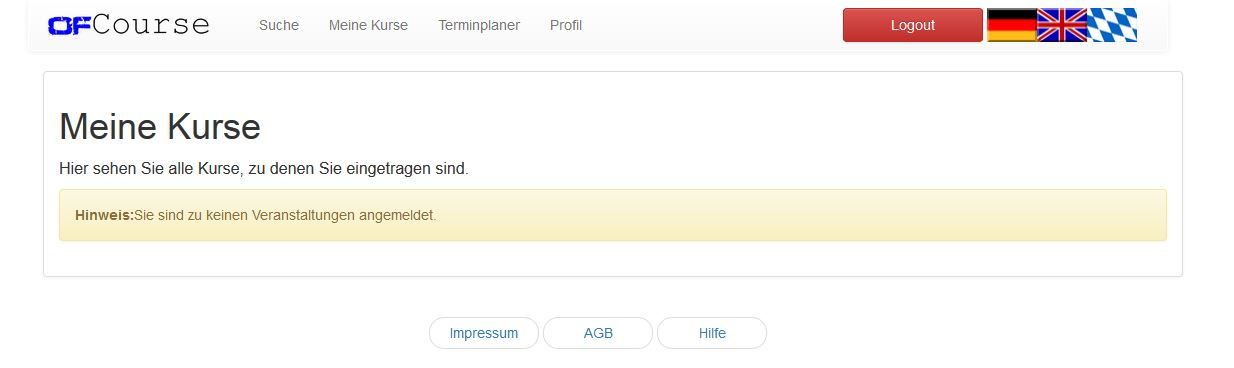
\includegraphics[width=0.8\linewidth]{Grafiken/myCoursesPage}
\caption{'Meine Kurse' - Seite von ofCourse}
\label{fig:myCoursesPage}
\end{figure}
\ \\
\ \\
\begin{center}
	{\Large Herzlich Willkommen bei \ \\}
	\ \\

\includegraphics[width=0.5\linewidth]{logo/name_blau_ofCourse}
\end{center}

\end{document}